\documentclass[conference]{IEEEtran}
\IEEEoverridecommandlockouts
% The preceding line is only needed to identify funding in the first footnote. If that is unneeded, please comment it out.
\usepackage{cite}
\usepackage{amsmath,amssymb,amsfonts}
\usepackage{algorithmic}
\usepackage{graphicx}
\usepackage{textcomp}
\usepackage{xcolor}
\usepackage{float}
\def\BibTeX{{\rm B\kern-.05em{\sc i\kern-.025em b}\kern-.08em
    T\kern-.1667em\lower.7ex\hbox{E}\kern-.125emX}}
\begin{document}

\title{Implementing Multi-Organizational Systems: Strategies and Ecosystems through Change Theory and Impact-Driven M\&E\\
{\footnotesize \textsuperscript{}}
\thanks{}
}

\author{\IEEEauthorblockN{Clément Combier}
\IEEEauthorblockA{\textit{Master 2 SIGLIS} \\
\textit{Université de Pau et des Pays de l'Adour}\\
Anglet, France \\
clement.combier@etud.univ-pau.fr}}
\maketitle

\section*{Abbreviation}
\begin{itemize}
    \item[] M\&E : Monitoring and Evaluation system 
    \item[] ToC : Theory of Change 
\end{itemize}

\begin{abstract}
This paper delves into the development of an impact-oriented Monitoring and Evaluation (M\&E) methodology within multi-organizational systems, inspired by the UNITA project – an innovative alliance of twelve European universities. Drawing on the principles outlined in Methods Lab's 'When and How to Develop an Impact-Oriented M\&E system' (2016), this study aims to rethink traditional M\&E approaches, emphasizing long-term impact and sustainable change.

We will use Theory of Change, which provide a structured framework to articulate and assess expected outcomes in complex collaborative environments. This approach is specifically interesting to our context of how inter-university collaborations can be optimized for greater effectiveness and increased impact.

Through practical examples and case studies, including those from the UNITA initiative, this paper illustrates the application of the Theory of Change in conjunction with impact-focused M\&E practices. The goal is to enhance goal alignment, communication, and the overall impact of joint initiatives.

In conclusion, this research offers new and practical perspectives for measuring and maximizing impact in complex collaborative settings. The study aims to illuminate pathways towards more effective and impactful multi-organizational collaborations.
\end{abstract}

\vspace{8pt}
\begin{IEEEkeywords}
Multi-Organizational Systems, Change Theory, Monitoring and Evaluation, M\&E, Impact-Driven Approach, Collaboration, Implementation Strategies, Organizational Ecosystems, Synergy, Communication in Multi-Organizational Settings, Alignment of Objectives, Shared Goals, Challenges in Implementation, Measuring Success, Lasting Change, Adaptability in Collaborations, Efficiency Metrics, Stakeholder Engagement, Inter-organizational Relationships, Framework for Impact Measurement, Best Practices in Multi-Organizational Collaborations.
\end{IEEEkeywords}
\vspace{16pt}

\section{Introduction}
\label{intro}
In a rapidly evolving global landscape, the need for effective multi-organizational systems has never been more apparent. This paper, inspired by the collaborative efforts within the UNITA project – an alliance of twelve European universities\cite{unita_unita_nodate}, seeks to develop an impact-focused Monitoring and Evaluation (M\&E) methodology. The UNITA project, with its commitment to inter-university cooperation and regional integration, serves as a prime example of the potential and challenges inherent in multi-organizational collaborations.

Drawing from the insights of the Methods Lab's 2016 paper, "When and How to Develop an Impact-Oriented M\&E system"\cite{hearn_when_2016}, this research aims to transcend traditional M\&E approaches. We focus on a broader perspective that emphasizes long-term impact and sustainable change, crucial for initiatives like UNITA.

The Theory of Change, is a structured way to understand the expected outcomes and impacts in complex collaborative environments. It is particularly relevant to the UNITA project, guiding our analysis on how inter-university collaborations could be optimized for greater effectiveness.

Through practical examples, including those from the UNITA initiative, this study illustrates the application of the Theory of Change in conjunction with impact-focused M\&E practices. We explore how these methodologies can improve goal alignment, communication, and the overall impact of joint initiatives.

The objective of this paper is to offer a critical examination of current M\&E methodologies in the context of multi-organizational systems like UNITA and to propose an enhanced framework that integrates the Theory of Change for more impactful evaluations.

In conclusion, this research contributes to the broader discourse on multi-organizational systems, providing new insights and practical approaches for measuring and maximizing impact. By focusing on projects like UNITA, we aim to shed light on the pathways to more effective and impactful multi-organizational collaborations.

\section{State of the Art}
\label{soa}
Reflecting on the UNITA project, the European University Initiative, launched in 2019 by the European commission, is a concrete case of the need for universities to cooperate together more than ever. This kind of project materialize the difficulty of a multi-organisation process to build communication system for all actors, through sometimes, different language, wide geographic area and much more factors that contribute to the complexity of the setup of this kind of project.\cite{european_commision_european_2019}
This first paper examined the European commission's European Universities Initiative plan \cite{european_commision_european_2019} and listed the potentials and perils of such project \cite{maassen_european_2023}. They have put in place a framework for analysing the promises and perils of this alliance. They used different field that could correlate to the alliance such as economic, environmental expectation and instrumental and network approaches.\cite{maassen_european_2023} To simplify the concept and to mutualize it to most fields, they've compared universities to meta-organization. \cite{maassen_european_2023} Meta-organization can be defined as :
\begin{quote}
    "Special kinds of organizations characterized by the fact that other organizations, and not individuals, account for the membership."
\end{quote}\cite{maassen_european_2023,gulati_meta-organization_2012,berkowitz_concept_2016,ahrne_meta-organizations_2008}.

An interesting methodology designed by Hearn et al. - 2016 - When and how to develop an impact-oriented monitor \cite{hearn_when_2016} using Theory of Change and M\&E system oriented impact for entire project and when and why to use this methodology.
\begin{figure}[H]
    \centering
    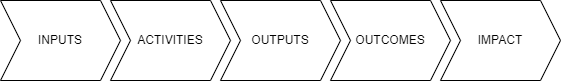
\includegraphics[width=1\linewidth]{res//diagrammes/impact_method_process.png}
    \caption{representation of a simplified results chain that includes impact\cite{hearn_when_2016}}
    \label{fig:enter-label}
\end{figure}
This methodology gives us a good starting point to further the research of this field within this paper. We start from the inputs, which represent the resources and materials needed to initiate a project or program to the impact, which represents the long-term effects and broader changes that occur as a result of the project, influencing stakeholders and the community.
Activities can be defined as specific actions and tasks performed to transform inputs into meaningful outcomes. These activities give us outputs or direct and immediate results of the activities, often quantifiable and measurable. Then, this outputs gives us outcomes, which indicate the initial achievements resulting from the outputs and activities, contributing to the project's objectives.
Using an impact approach can be very benefic to big project spanning across meta-organizations. It allows for a bigger picture at the end, and not just the scope of the outcomes of the project (as most project are usually being developed). Impact allows forces us to see into the future and what it could hold for the organizations and how it would \textbf{impact} the world.
This paper also mentions the use of Theory of Change, which is a way to describe initiative or program logic. The process when employing ToC is to see the long-term effects awaited by the project, then map backward the entire process to start \textit{inputs} from the theory envisioned for the project.\cite{taplin_toc-tech-papers_imppdf_2013}.
In their conclusion, the authors have made it clear that not every project need to have that scope for the future. They give out specific rules that can be applied to tell if a project may need impact oriented approaches or not. 
\begin{quote}
    \begin{enumerate}
        \item information	about	 impact	will	be	useful	and	timely	to	support	specified	 decision-making	needs;
        \item impact	is	deemed	plausible	 and	is	feasible	to	assess	with	rigour;
        \item resources	 and	capacity	for	collecting,	analysing	and	interpreting	 impact	data	are	adequate.
    \end{enumerate}		
\end{quote}
Also, it is important to use ToC when building a M\&E system when it is impact oriented. This \textit{tool} will considerably help design and build the system, processes, policies, etc.\cite{hearn_when_2016}

\subsection{Conclusions} 

\section*{Acknowledgment}
\vspace{12pt}
\bibliographystyle{plain}
\bibliography{bib/references}

\end{document}
